\chapter{Introduzione}

Nel panorama odierno della sicurezza informatica, ogni secondo conta. Quando un sistema viene compromesso, gli attaccanti lasciano tracce invisibili che esistono solo nella memoria volatile del computer - tracce che svaniscono al riavvio del sistema. È in questo contesto che la Digital Forensics e, in particolare, l'analisi della memoria, assumono un ruolo fondamentale nella risposta agli incidenti e nelle investigazioni digitali.

\section{Contesto e Motivazioni}

\subsection{L'importanza crescente della Digital Forensics nell'era digitale}

Viviamo in un'epoca in cui la trasformazione digitale ha permeato ogni aspetto della società. Dalle infrastrutture critiche ai servizi finanziari, dalla sanità alla difesa nazionale, la dipendenza dai sistemi informatici è totale e irreversibile. Questa digitalizzazione pervasiva ha però un lato oscuro: l'espansione della superficie di attacco e la crescente sofisticazione delle minacce cyber.

Secondo il rapporto Clusit 2025 \cite{clusit2025}, gli attacchi informatici sono aumentati del 27\% a livello globale e del 15\% in Italia rispetto all'anno precedente, con danni economici stimati in miliardi di euro.

\begin{figure}[ht]
    \centering
    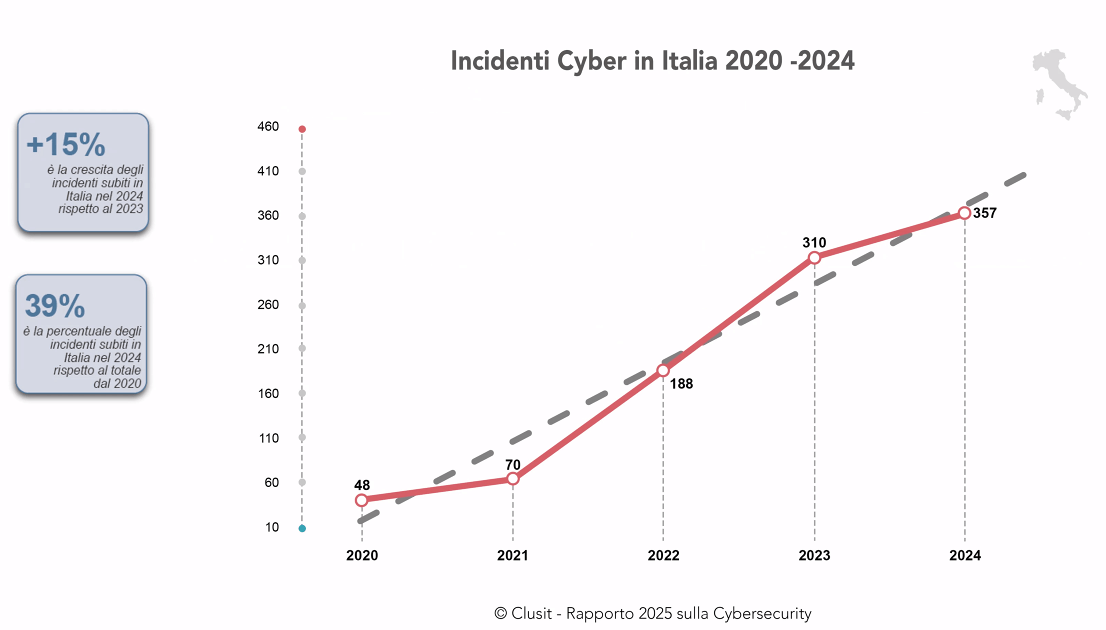
\includegraphics[width=1\linewidth]{images/intro/clusit-ita.png}
\end{figure}

In questo scenario, la Digital Forensics non è più una disciplina di nicchia riservata alle forze dell'ordine o all'applicazione in ambito strettamente militare, ma è una competenza essenziale per qualsiasi organizzazione che voglia proteggere i propri asset digitali e rispondere efficacemente agli incidenti di sicurezza.

La Digital Forensics, definita come "l'applicazione di tecniche scientifiche per l'identificazione, raccolta, analisi e presentazione di evidenze digitali in modo che siano ammissibili in tribunale" \cite{palmer2001}, si è evoluta ben oltre il suo scopo originario. Oggi, il Digital Forensics and Incident Response (DFIR) rappresenta un pilastro fondamentale della cybersecurity aziendale, fornendo le capacità necessarie per:

\begin{itemize}
   \item \textbf{Rilevare} attività malevole che i sistemi di sicurezza tradizionali potrebbero aver mancato
   \item \textbf{Comprendere} la portata e l'impatto di un incidente di sicurezza
   \item \textbf{Contenere} la minaccia e prevenire ulteriori danni
   \item \textbf{Recuperare} i sistemi compromessi e ripristinare le operazioni normali
   \item \textbf{Apprendere} dall'incidente per migliorare le difese future
\end{itemize}

\subsection{Il ruolo critico dell'analisi della memoria nei processi investigativi}

Tra le varie tecniche di Digital Forensics, l'analisi della memoria RAM occupa una posizione privilegiata. A differenza dell'analisi del disco, che esamina dati persistenti, l'analisi della memoria cattura lo stato ``vivo'' del sistema al momento dell'acquisizione, rivelando:

\begin{itemize}
   \item \textbf{Processi in esecuzione}: inclusi quelli nascosti o offuscati dai rootkit
   \item \textbf{Connessioni di rete attive}: fondamentali per identificare comunicazioni con server di comando e controllo
   \item \textbf{Chiavi crittografiche}: spesso presenti solo in memoria durante l'uso
   \item \textbf{Artefatti di malware}: codice iniettato, hook di sistema, modifiche alle strutture del kernel
   \item \textbf{Credenziali in chiaro}: password e token di autenticazione temporaneamente decriptati
\end{itemize}

L'importanza dell'analisi della memoria è cresciuta esponenzialmente con l'evoluzione delle tecniche di attacco. I moderni malware sono progettati per operare esclusivamente in memoria (fileless malware), lasciando poche o nessuna traccia sul disco. Tecniche come process injection, reflective DLL injection e living-off-the-land rendono l'analisi della memoria non solo utile, ma spesso l'unico modo per rilevare e comprendere un attacco sofisticato.

\subsection{Sfide attuali}

Nonostante la sua importanza critica, l'analisi della memoria continua a incontrare ostacoli significativi che ne limitano la diffusione su larga scala. In primo luogo, si tratta di un ambito con una complessità tecnica molto elevata: richiede una conoscenza approfondita delle strutture interne del sistema operativo, dei meccanismi di gestione della memoria e delle svariate tecniche di anti-forensics adottate dai malware moderni. Questa curva di apprendimento particolarmente ripida tende a scoraggiare molti professionisti della sicurezza, che preferiscono focalizzarsi su domini più consolidati come l’analisi di file system o di log di rete.

A questo si aggiunge il problema del volume dei dati. I sistemi attuali possono disporre di decine o addirittura centinaia di gigabyte di RAM, rendendo impraticabile un’analisi manuale senza l’ausilio di strumenti automatizzati e tecniche di filtraggio avanzate in grado di isolare rapidamente gli artefatti di interesse.

Un’ulteriore criticità è data dalla natura intrinsecamente volatile della memoria: ogni secondo che passa dopo un incidente aumenta il rischio che evidenze cruciali vengano sovrascritte o vadano perse. Questo introduce un forte vincolo temporale nelle attività di incident response, imponendo procedure di acquisizione che siano al tempo stesso rapide ed estremamente affidabili.

Dal punto di vista strumentale, l’ecosistema delle soluzioni per la memory forensics è ancora frammentato. Il framework open source Volatility rappresenta lo standard di fatto, ma richiede competenze da linea di comando e restituisce output che devono essere interpretati con grande esperienza. Altre soluzioni, tipicamente commerciali, spesso hanno costi elevati e funzionalità che non sempre giustificano l’investimento.

La mancanza di automazione rappresenta un’altra sfida non trascurabile. Molte operazioni, dall’identificazione dei pattern sospetti alla correlazione tra artefatti e alla stesura dei report, restano attività manuali e time-consuming, drenando tempo e risorse che potrebbero essere dedicate all’analisi strategica delle minacce.

Infine, integrare i risultati dell’analisi della memoria con altre fonti di intelligence — come log applicativi, traffico di rete o feed di threat intelligence — rimane un processo in larga parte artigianale e suscettibile di errori, compromettendo la visibilità complessiva dell'incidente.

È proprio per rispondere a queste sfide che nascono piattaforme come VolWeb \cite{volweb2024}, concepite per democratizzare l’accesso alla memory forensics attraverso interfacce intuitive, automazioni intelligenti e capacità di correlazione avanzate, riducendo drasticamente la barriera d’ingresso e aumentando l’efficacia delle investigazioni.

\section{Obiettivi della Tesi}

Questo lavoro di tesi si propone di affrontare le sfide identificate attraverso l'espansione e il miglioramento di VolWeb, una piattaforma web-based per l'analisi forense della memoria. Gli obiettivi specifici sono:

\subsection{Integrazione di YARA nella piattaforma}

L’obiettivo principale è integrare un sistema completo per la gestione e l’applicazione di regole YARA, strumento fondamentale per l’identificazione di pattern e malware nei dump di memoria. Questa integrazione mira a:

\begin{itemize}
\item Gestione centralizzata, creazione e validazione delle regole YARA direttamente da VolWeb;
\item Applicazione efficiente delle regole su dump di memoria durante le analisi forensi;
\item Visualizzazione e reportistica dei risultati derivanti da YARA per facilitare l’interpretazione da parte degli analisti.
\end{itemize}

\subsection{Validazione in contesti operativi reali}

Il secondo obiettivo è validare e ottimizzare l’uso di VolWeb con la nuova integrazione YARA in scenari operativi reali, con particolare attenzione a:

\begin{itemize}
\item Preparazione per l’utilizzo nell’esercitazione NATO CCDCOE Locked Shields 2025, il più grande esercizio di cyber defense a livello mondiale;
\item Stress test della piattaforma in condizioni di carico elevato, con analisi concorrenti di dump multipli;
\end{itemize}

Questi obiettivi non sono meramente tecnici, ma rispondono a un'esigenza concreta del mondo della cybersecurity: rendere l'analisi della memoria accessibile, efficiente e integrata nel workflow di incident response moderno.